\documentclass[10pt]{beamer}

\usetheme{CambridgeUS}
\usepackage[english, russian]{babel}
\usepackage[utf8]{inputenc}
\usepackage{caption}
\usepackage{etoolbox}
\usepackage{multicol}
\usepackage{listings}
\usepackage{color}

\definecolor{mygreen}{rgb}{0,0.6,0}
\lstset{
  basicstyle=\ttfamily\footnotesize,        % the size of the fonts that are used for the code
  breaklines=true,                 % automatic line breaking only at whitespace
  captionpos=b,                    % sets the caption-position to bottom
  commentstyle=\color{mygreen},    % comment style
  keywordstyle=\color{blue},       % keyword style
  stringstyle=\color{red},     % string literal style
  showstringspaces=false,
  morekeywords={include, printf},
  texcl=true     %<---- added
  numbersep=14pt
}

\title[\href{https://goo.gl/NRgp8K}{https://goo.gl/NRgp8K} (Term 3)]{Суфф. дерево. Алгоритм Укконена}
\author[Зацепин Михаил]{Зацепин Михаил}
\institute[МФТИ] 
{Московский физико-технический институт\\*}
\date{Москва, 2018}
\subject{Computer Science}

\begin{document}

\begin{frame}
  \titlepage
\end{frame}

\section{Суффиксное дерево}
\begin{frame}[fragile]{Определение}
Суффиксное дерево для строки \texttt{s} (\texttt{m = |s|}) - дерево с \texttt{m} листьями:
\begin{itemize}
\item{У каждой внутренней вершины не меньше 2 детей}
\item{Каждое ребро помечено непустой подстрокой \texttt{s}}
\item{Никакие два ребра, выходящие из одной вершины, не могут иметь пометок, начинающихся с одного и того же символа}
\item{Каждый суффикс строки заканчивается в листе и только в нем}
\end{itemize}
\end{frame}

\section{Суффиксное дерево}
\begin{frame}[fragile]{Пример}
Дерево для строки \textcolor{red}{a}
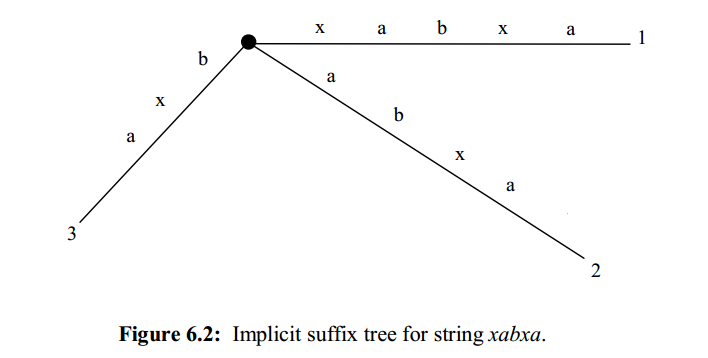
\includegraphics[scale=0.5]{Term_3/Source/Pictures/Implicit_Suff_Tree.png}
\end{frame}

\section{Суффиксное дерево}
\begin{frame}[fragile]{Пример}
Дерево для строки \textcolor{red}{a}
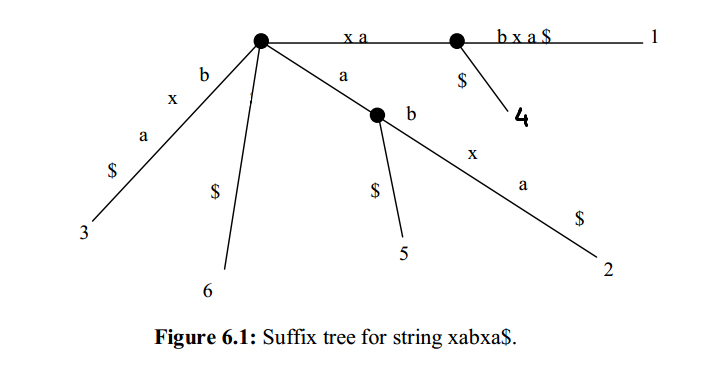
\includegraphics[scale=0.5]{Term_3/Source/Pictures/Suff_Tree.png}
\end{frame}

\section{Суффиксное дерево}
\begin{frame}[fragile]{Наивный алгоритм}
\end{frame}

\section{Алгоритм Укконена}
\begin{frame}[fragile]{Алогритм Укконена}
\end{frame}

\end{document}